\documentclass[10pt]{sensys-proc}

\usepackage{balance}
\usepackage{graphicx}
\usepackage{url}

\crdata{978-1-4503-1169-4}
\conferenceinfo{PhoneSense'12,} {November 6, 2012, Toronto, ON, Canada.}
\CopyrightYear{2012}

\numberofauthors{2}

\author{
\alignauthor Kasturi Rangan Raghavan, Supriyo Chakraborty, Mani Srivastava\\
	\affaddr{University of California, Los Angeles}\\
	\email{\{kasturir,supriyo,mani\}@ucla.edu}
\alignauthor Harris Teague\\
	\affaddr{Qualcomm Inc.}\\
	\email{hteague@qualcomm.com}
}

\title{\textsc{Override}: A Mobile Privacy Framework for Context-Driven
Perturbation and Synthesis of Sensor Data Streams}

\begin{document}

\maketitle

\begin{abstract}
Smart phones with increased computation and sensing capabilities have spurred the growth of context-aware apps. Apps have direct access to raw sensor data streams, and can use them to infer a user's personal context. Although an app may provide a useful advertised service in return, the sharing of raw sensor data with a malicious app allows it extract other sensitive information. Something that is considered private by the user. Current approaches to mitigate such privacy concerns rely on simple user-specified policies consisting of static rules and amounts to all-or-nothing access to sensor data. Such rules are conservative and contribute to a sharp decline in an app's usefulness. In this paper we address the challenge of balancing user privacy and application utility. To this end, we present \textsc{Override}: a mobile privacy framework that empowers users to specify context-driven rules to control the sensor data delivered to an app. It supports fine-grained control mechanisms including context-driven suppression, perturbation, and synthesis of sensor data streams. We discuss the architecture of \textsc{Override} and describe a prototype implementation of it on the Android platform. We highlight the framework's ability to provide users with increased transparency and control over shared sensor data.
\end{abstract}

\section{Introduction}
\label{sec:intro}
Smart phone apps are increasingly context-aware and rely on having access to raw sensor data streams to infer personal context. The usual benefit of context-aware apps is that they offer tailored, personalized services. On the other hand, a mobile platform that so liberally provides apps access to sensor data leaves open room for abuse; a malicious app can use the same sensor data to extract sensitive information that is considered private by the user. Seemingly innocuous sensor measurements can be used to make surprisingly sensitive inferences about the user. Many sensitive inferences and longer-term profiling of sensitive behaviors are possible from shared location data. ~\cite{krumm:survey} provides a survey. A special concern is with external physiological sensors, since many sensitive inferences about medical conditions become possible. For instance,~\cite{plarre:psychological,rahman:mConverse,Ertin:AutoSense} have demonstrated reliable inferences of psychosocial stress and smoking habits from a respiration sensor. Since physiological sensors may become standard on next-generation mobile devices, we believe its worthwhile exploring context-driven privacy mechanisms controlled dissemination of sensor data.

The security mechanisms in current mobile platforms require that applications declare the sensors that they will use during install time. We believe such basic mechanisms are inadequate, and in stark contrast to a user's true privacy requirement. The binary choice presented to the user is entirely unsatisfactory: the app can be installed with the requested permissions or not installed at all. An app may advertise a service that justifies its request for sensor data, but access to raw sensor data is usually unnecessary. Ideally the users wants some assurance that an app uses the sensor data appropriately for only the advertised service and that the app is not collecting sensor data to make sensitive inferences. Current mobile platforms have the ability to only provide raw sensor data and so all current apps operate on raw sensor data streams. The mobile platform does not understand the app's intent for requesting sensor data, and so is unable to determine whether coarser granularity data stream is sufficient. Thus the mobile platform lacks the knowledge and ability to identify malicious apps that misuse their access to sensor data streams by making unadvertised sensitive inferences.

One solution is to limit the sensitive information that apps can extract from sensor data in the first place. In this paper we adopt this mindset, and take some initial steps towards curbing the ability of apps to make sensitive inferences. We observe that privacy requirements are better expressed in terms sensitive personal contexts. For instance, an inference that can be made from location data is to infer the places that a user visits. All places are not uniformly sensitive, there may be specific places like hospitals and places of worship that reveal something personally sensitive like medical conditions or religion, respectively.

We propose \textsc{Override} a mobile privacy framework which provides users with the ability to specify context-dependent privacy policies that supports suppression, perturbation, or even synthesis of sensor data streams. With the framework we can perform privacy-preserving operations whenever the user is inferred to be in a sensitive context such a sensitive location. We propose such context-driven privacy policies as a means to limit the sensitive information delivered to untrusted and possibly malicious apps. We describe the architecture of \textsc{Override} and present a prototype implementation on Android that implements a secure mechanism for intercepting the delivery of sensor data to apps, enabling context-driven operations to be performed on sensor data streams before it is delivered to apps.

The rest of the paper is organized as follows. The high-level design of the \textsc{Override} framework, and the implementation details on the Android mobile platform are presented in Section~\ref{Sec:architecture}. In Section~\ref{Sec:example} we outline an example scenario to demonstrate how \textsc{Override} can be leveraged for location privacy. Related work is summarized in Section~\ref{Sec:related}, followed by a summary of the work in Section~\ref{Sec:conclusion}.

\section{The \textsc{Override} Framework}
\label{Sec:architecture}
\begin{figure}
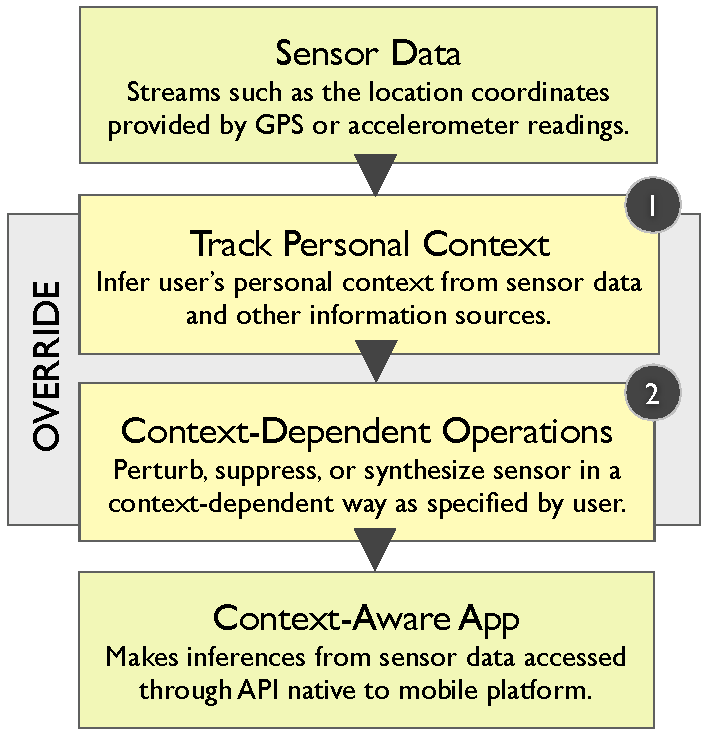
\includegraphics[width=\columnwidth]{../figures/flow5.pdf}
\caption{The key functionality of the \textsc{Override} framework.}
\label{fig:flow}
\end{figure}

We first provide a high-level overview of \textsc{Override}, and then in Section~\ref{sec:implementation} discuss the details of a prototype implementation on the Android mobile platform. As visualized in Figure~\ref{fig:flow} the core functionality of \textsc{Override} is to deliver suitably processed sensor data streams to apps and facilitate context-driven privacy policies. This is achieved by tracking the personal context of a user (\emph{Track Personal Context}) and then applying suitable context-dependent privacy transformation on the stream (\emph{Context-Dependent Operations}). \textsc{Override} allows sensor data streams to be processed differently and specifically for each app that requests sensor data, enabling targeted dissemination of sensor data.

\subsection{Design Overview}

We briefly discuss tracking personal context, and then discuss broad categories of data processing operations that can be driven by personal context. More concrete applications of context-driven operations are left for Section~\ref{Sec:example}.

\subsubsection{Tracking Personal Context.}

An external context-providing service is instantiated and left to run in the background. The service makes various contextual inferences from sensor data and from other information sources. For example, the service may make two contextual inferences: (1) user activity, and (2) indoor or outdoor. Say the former inference classifies the user's current activity into one of $\{Still, Running, Walking\}$, and that the output of the latter inference takes on one value from $\{Indoor, Outdoor, Uncertain\}$. We abstract away from the implementation details of these inferences, since \textsc{Override} does need that information. Together these inferences determine the user's personal contextual state at any point in time, and \textsc{Override} is able to track that with the help of the context-providing service.

\subsubsection{Context-Dependent Operations.}
We permit standalone, externally-implemented modules to provide \textsc{Override} with processed sensor data streams. In this way, we can readily integrate different data processing operations. The operates we support include:

\textbf{Perturbation and Adding Noise.} We support standard mechanisms that are known to lower the quality of the sensor data signals as a means to enable privacy. For example, location coordinates can be quantized to lower the spatial resolution. Accelerometer data can be sub-sampled or otherwise filtered as a means to sanitize the signal.

\textbf{Suppression.} Compared  to perturbation which delivers lower quality sensor data to apps, suppression entirely blocks the delivery of sensor data. For instance, suppression blocks the delivery of GPS location coordinate streams, mimicing the behavior observed in the the event that GPS sensor is turned off.

\textbf{Context-Driven Sensor Data Synthesis.} Besides perturbation and suppression, a third technique we consider to facilitate privacy is sensor data synthesis. See Section~\ref{Sec:related} for prior work that has used synthetic sensor data for privacy. The novelty of our approach is that we consider driving the synthesis of sensor data based on the current personal contextual state.

\subsection{A Prototype Android Implementation}
\label{sec:implementation}
We implemented the \textsc{Override} framework in Java within the Android mobile platform. Parts of the underlying architecture was inspired by PDroid~\footnote{Available at \url{https://play.google.com/store/apps/details?id=com.privacy.pdroid}}, an open-source framework for implementing static sensor access control policies. The components of the full \textsc{Override} implementation are shown in Figure~\ref{fig:android_impl}.

In this paper, we focus on the implementation details of the \texttt{OverrideDataManager}. It makes up the main modification we have made to the Android platform, and it is the component that enables the delivery of processed sensor data streams to apps. Our system is loosely coupled and extensible, allowing third parties to integrate with \textsc{Override} and provide it with privacy-preserving sensor data streams that can be relayed to apps. In Section~\ref{Sec:example} we discuss in detail how to leverage our framework as a location privacy platform.

\begin{figure}
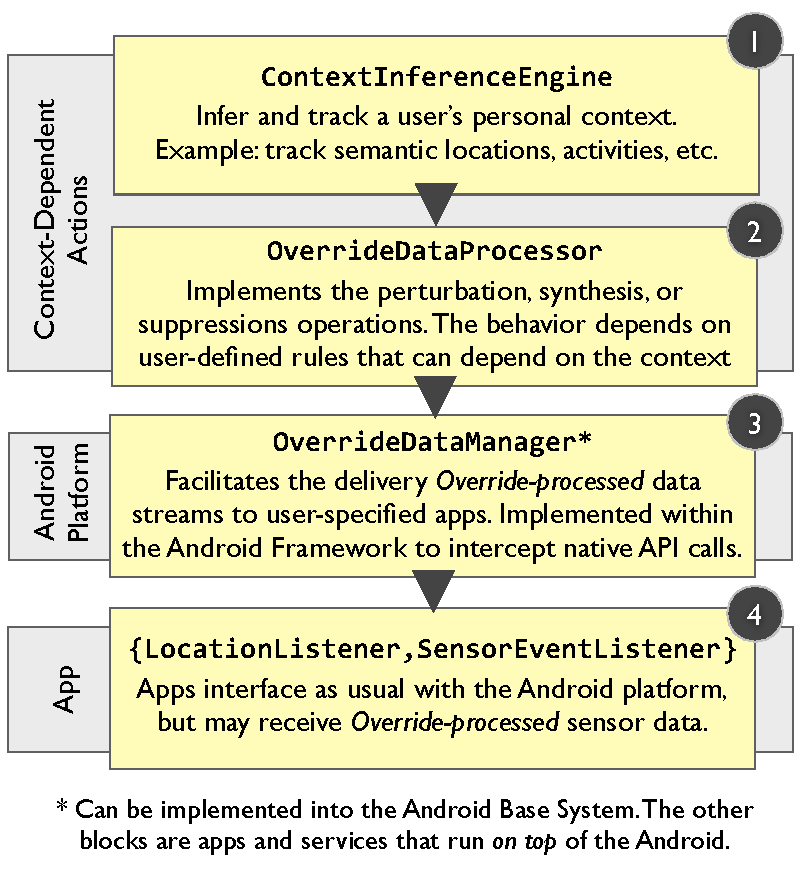
\includegraphics[width=\columnwidth]{../figures/android_impl4.pdf}
\caption{The data flow in the \textsc{Override} Android Implementation}
\label{fig:android_impl}
\end{figure}

\textbf{Replacing the Android LocationManager and SensorManager.} The Android platform maintains system services that manage the pushing of sensor data streams to apps. We consider the capability to process two such Android-provided sensor data streams: (1) location updates managed by the \texttt{LocationManager} and (2) \emph{sensor} updates managed by the \texttt{SensorManager}. The former provides apps that request location coordinates from GPS, WiFi-based, and cell-network sources. The latter provides apps that request accelerometer, gyroscope, and magnetic (compass) measurements, and other sensors. In the future we would like to consider intercepting and then processing image and audio data before they are delivered to apps, and also consider other non-sensory data streams like calendar events which apps are allowed unrestricted access with the appropriate permissions.

Android apps follow a straightforward protocol to request sensor data streams. An app first obtains a handle to one of the aforementioned \texttt{Manager} services, and then registers with it a data listener object. Registered listeners will then asynchronously receive location or sensor data.

We implement an \texttt{OverrideDataManager} system service that exposes the same API to apps as the existing \texttt{Manager} services, and effectively replaces them. When apps attempt to obtain a handle one of the native \texttt{SensorManager} or \texttt{LocationManager} services, we produce instead a handle to \texttt{OverrideDataManager}. In this way, \textsc{Override} owns all registered sensor data listeners, and enables full targeted control over the sensor data delivered to each app.
 
\textbf{Standalone Services to Provide Sensor Data Streams.} Analogous to the way that the native Android \texttt{LocationManager} permits externally-implemented and proprietary providers of location data, our \texttt{OverrideDataManager} exposes a simple API that permits external, standalone Android ``provider'' services to report custom location and sensor data streams. In this way, the \texttt{OverrideDataManager} can accept perturbed or synthetic sensor data streams. We have implemented standard perturbation and synthesis services for location and accelerometer data, but this functionality can also be implemented by a third party developer, and distributed to users on the app-store.

\textbf{Mapping Available Sensor Data Streams to Apps.} We have built a central, user-configurable system service called the \texttt{OverrideSettingsManager}, and it's not shown in Figure~\ref{fig:android_impl}. This central service facilitates two decisions. First, a user will not usually configure every apps to receive processed sensor data, and so only those apps specifically designated will receive custom sensor data streams.  All other apps will continue to receive unprocessed raw sensor data. Second, since we allow standalone ``provider'' services, the \texttt{OverrideSettingsManager} maintains the mapping that specifies which apps should receive which custom sensor data streams.

In the current prototype implementation, the context-dependent behavior of the custom sensor data streams is left up to the implementation of the standalone ``provider'' services. In future versions, we imagine users will be able centrally configure context-dependent behavior within the \texttt{OverrideSettingsManager}.

\section{Examples of Context-Driven Privacy}
\label{Sec:example}

We discuss some concrete applications of context-driven privacy policies, especially as a way for users to more transparently express privacy requirements for location privacy and in other settings. We briefly discuss potential secondary benefits that we leave as future directions for research.

\subsection{Location Privacy}

Location-aware services have become very popular, increasingly so with the advent of ``check-in'' services by social networks. Naturally location is a valuable signal that's useful for pulling in local traffic, new, weather updates, and to automatically geo-tag photos when sharing them. From the user's perspective, visualizing and controlling which apps receive what location updates can promote a sense of privacy. There's a large amount of work in literature that addresses the issue of location privacy~\cite{krumm:survey}, and many focus on lowering the quality of the provided location coordinates by decreasing it's resolution or adding structured noise. In this section, we demonstrate how \textsc{Override} can be leveraged to deliver custom, privacy-preserving location coordinate streams to existing location-aware apps.

\begin{figure}[h]
\label{fig:semantic_places}
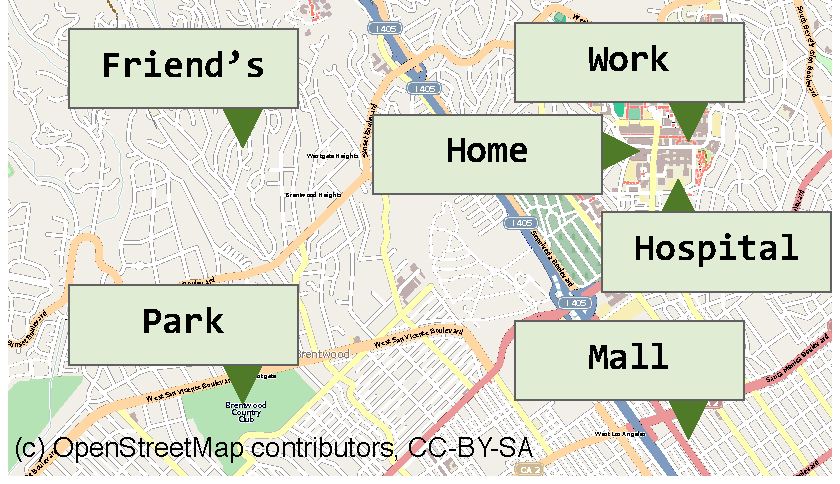
\includegraphics[width=\columnwidth]{../figures/semantic_location_3.pdf}
\caption{A set of semantic places with names and geo-tagged by the user that supplements GPS location.}
\end{figure}

\textbf{Semantic Locations.} In particular, we consider using \textsc{Override} as a mechanism to replace the conventional GPS-derived location coordinates with \emph{semantic locations}. Semantic locations are places that are personally meaningful to the user. The user maintains a geo-tagged set of semantic locations; see Figure~\ref{fig:semantic_places} for an example. GPS-derived location coordinates can be used to infer the user's current semantic location.

The primary privacy benefit that results from sharing semantic locations arises from the fact that semantic locations are meaningful to the user and only a certain set of locations are allowed to be shared with an app. When the user configures \textsc{Override} to deliver semantic locations to apps in lieu of GPS-derived location, these apps will begin to receive location coordinates that jump between the user's configured semantic locations as the user moves between them. If the user is not in a valid semantic location or if that semantic location is not allowed to be shared with an app, then \textsc{Override} can be setup to either suppress location updates or provide updates that correspond to the location of the previously visited and allowed semantic location.

We will now describe at a high level an instantiation of \textsc{Override} to incorporate semantic location updates delivered to apps. We follow the proposed Android architecture from Section~\ref{sec:implementation}; in particular, following the component-level description in Figure~\ref{fig:android_impl}. Consider the semantic location inferences are implemented by a standalone Android service. This service provides a UI to allow the user to maintain the list of geo-tagged semantic locations, and it reports to the \texttt{OverrideDataManager} the user's semantic location as it is changes over time. In this system, we have combined the functionality of the \texttt{ContextInferenceEngine} and \texttt{OverrideDataProcessor} blocks from Figure\ref{fig:android_impl} into a monolithic standalone service. We can think of the semantic locations as a context-dependent perturbation operation on the original GPS-derived location coordinates. This service periodically pushes location updates in the form of (latitude, longitude) coordinates to the \texttt{OverrideLocationManager}. Finally, a separate UI as provided by the\texttt{OverrideSettingsManager} allows the user to specify which app should receive semantic location updates in lieu of GPS-derived location. With the aforementioned configuration in place, \textsc{Override} will ensure that the designated apps will receive the semantic location updates.

\textbf{\textsc{Override} as a location privacy platform.} The uses of \textsc{Override} are not limited to providing only semantic locations. Note that at any one time there can be a number of active custom location providers, each implemented as standalone service and providing a different context-dependent, privacy-preserving location coordinate stream. A second location provider in addition to the semantic location provider previously described may provide a coarser-grained zip-code resolution location coordinate stream. A location-aware weather application can be configured to receive location coordinates from this provider since all the weather application really needs is something with zip-code level resolution, and provided with a coarser-grained locations stream the weather app is prevented from making sensitive inferences from location which often require access to more fine-grained location data. In this way, more straightforward privacy policies such as geo-fencing apps to receive location updates only within a certain geographical area can be realized. \textsc{Override} can serve as a location-privacy platform that empowers users to to curb apps' ability to make unadvertised and possibly sensitive inferences. We want to implement in the future more sophisticated context-driven suppression mechanisms such as that in~\cite{Gotz:MaskIt}.

\subsection{Context-Driven Accelerometer Policies}
\textbf{Suppression.} \textsc{Override} can also be leveraged to address other privacy concerns besides location privacy. In our implementation we also have the ability to override the others sensors that exist in Android. In particular, the onboard accelerometer sensor is a popularly used sensor that is used by many fitness and wellness apps as a means track activity levels. Recently, we have seen some work that revealed a user's keyboard strokes on the phone's soft keyboard can be deciphered from capturing only the accelerometer data from the onboard sensors~\cite{Keyboard}. To alleviate such concerns, \textsc{Override} can be configured to suppress accelerometer data to all apps whenever the soft keyboard is visible on the screen. As an alternative to suppression, we can configure \textsc{Override} to to add Gaussian noise to the accelerometer data whenever the software keyboard is visible.

\textbf{Synthesized data that preserves certain features.} In addition, we can synthesize sensor data that preserves only specific statistical properties of the actual observed signal as a means of enabling only a specific application utility. For instance, we can deliver synthetic accelerometer data to an accelerometer-based pedometer app where the synthetic data has the same variance as the actual accelerometer sensor data stream, but otherwise the synthesized stream is drawn from maximum-entropy distribution. This way the pedometer app can continue to operate with some degradation in utility--counting steps taken or activity level. However, the synthetic data does not contain enough information to make sensitive inferences like inferring specific activity types~\cite{Fusion}.

\subsection{Secondary Benefits Besides Privacy}
Higher-level contextual inferences can often supplement sensor data streams, making them more accurate or more available. For example, GPS is a very accurate sensor of location. This sensor works great outdoors, but the signal is often unavailable indoors. To combat this weakness, the research community have proposed various effective alternatives that can infer location when GPS is not available. For instance, in the previous section we discussed the inference of semantic locations using GPS as the primary sensor. However, these semantic locations can also be inferred via WiFi and Bluetooth landmarks~\cite{Kim:PlaceSens,Ananthanarayanan:BlueFi}, and interestingly such a semantic location inference is often most useful indoors. A custom \textsc{Override} location provider that incorporates such improvements can provide existing apps with more comprehensive and energy-efficiently derived location coordinate stream resulting in increased application utility.

\section{Related Work}
\label{Sec:related}
It is well known that mobile phone sensor data can be used to make a rich set of inferences about personal context and behavior. More recent work in this space have even explored using collaborative inference algorithms and information fusion for improved inferences~\cite{Miluzzo:DarwinPhones}. There's been much work on designing mobile platforms that have built-in services that can provide apps with \emph{contextual inferences} directly. This line of thinking is a natural progression of mobile platform design, see~\cite{Raento:ContextPhones} or more recently~\cite{Chu:CondOS} for an overview of two architectures. However, current mobile platforms do not incorporate such architectures, and apps must resort to operating on sensor data, even if internally a context-providing library is used to make appropriate inferences.

Sharing \emph{contexts} with apps instead of the sensor data is useful for controlled context release. This way, the mobile platform can inform the user more precisely what is being shared, it increases the transparency of what's shared and it is useful for privacy. However, many existing apps do not make use of context-providing libraries, and neither context-providing libraries nor typical context-aware apps expose any user interface that allows users to control the types of inferences being made from sensor data. Unless current mobile platforms incorporate provide high-level context directly, apps will remain to operate directly on sensor data. The work in this paper presents a framework that's practical to implement on current mobile platforms and does not require that apps use a special context-providing library. This work represents a solution that enables users to control the the many existing apps that operate directly on sensor data.

There is prior work on tracking when and what sensor data is accessed, providing capabilities beyond what exists in the current mobile platforms. Some such systems allow the user to limit an individual app's access to sensor data, or let users configure it to send a fixed synthetic value~\cite{Beresford:MockDroid,Enck:TaintDroid}. These works we classify as basic access control and information flow mechanisms applied to sensor data sources. They are limited to providing users with static policies. For example, \cite{Beresford:MockDroid} enable a user to setup a rule such that an app always receives a fixed location value. The work presented in this paper is complimentary to previous work. To the best of our knowledge, we have not seen before the idea of using personal context to \emph{drive} the perturbation or synthesis of sensor data. Other approaches taken for privacy consider suppressing \emph{sensitive} contexts and some systems even attempt to block \emph{inference of sensitive contexts}~\cite{Gotz:MaskIt}, but these are just studies and they are not implemented as true mobile frameworks. We imagine system architectures such as \textsc{Override} can facilitate the aforementioned privacy mechanisms, but we leave a thorough evaluation to future work.

%Closest in functionality to \textsc{Override}, is Protect-My-Privacy (PMP)~\cite{pmp}. However, implemented on the iOS platform, PMP is designed for non-sensory non-time series data and focuses on tracking surreptitious and unadvertised access by applications to information sources which may have private information but which iOS allows any application to access.

\section{Summary}
\label{Sec:conclusion}
We presented \textsc{Override}, a privacy framework that allows users to exercise fine-grained context-aware control over the sensory data being shared with various untrusted applications. \textsc{Override} provides this functionality by intercepting the sensor data requests from applications and applying user specified privacy-preserving transformations such as perturbation and suppression of data, or synthesis of data streams before sharing. We provided a prototype implementation of the framework and used a location sharing based application scenario to illustrate the ease of application development using the framework.

\balance
\bibliographystyle{abbrv}
\bibliography{override}
\end{document}
